\documentclass[
  shownotes,
  xcolor={svgnames},
  hyperref={colorlinks,citecolor=DarkBlue,linkcolor=andesred,urlcolor=DarkBlue}
  , aspectratio=169]{beamer}
\usepackage{animate}
\usepackage{amsmath}
\usepackage{amsfonts}
\usepackage{amssymb}
\usepackage{pifont}
\usepackage{mathpazo}
%\usepackage{xcolor}
\usepackage{multimedia}
\usepackage{fancybox}
\usepackage[para]{threeparttable}
\usepackage{multirow}
\setcounter{MaxMatrixCols}{30}
\usepackage{subcaption}
\usepackage{graphicx}
\usepackage{lscape}
\usepackage[compatibility=false,font=small]{caption}
\usepackage{booktabs}
\usepackage{ragged2e}
\usepackage{chronosys}
\usepackage{appendixnumberbeamer}
\usepackage{animate}
\setbeamertemplate{caption}[numbered]
\usepackage{color}
%\usepackage{times}
\usepackage{tikz}
\usepackage{comment} %to comment
%% BibTeX settings
\usepackage{natbib}
\bibliographystyle{apalike}
\bibpunct{(}{)}{,}{a}{,}{,}
\setbeamertemplate{bibliography item}{[\theenumiv]}

% Defines columns for bespoke tables
\usepackage{array}
\newcolumntype{L}[1]{>{\raggedright\let\newline\\\arraybackslash\hspace{0pt}}m{#1}}
\newcolumntype{C}[1]{>{\centering\let\newline\\\arraybackslash\hspace{0pt}}m{#1}}
\newcolumntype{R}[1]{>{\raggedleft\let\newline\\\arraybackslash\hspace{0pt}}m{#1}}


\usepackage{xfrac}


\usepackage{multicol}
\setlength{\columnsep}{0.5cm}

% Theme and colors
\usetheme{Boadilla}

% I define a custom pallete
\definecolor{andesred}{HTML}{1B175E}
\definecolor{andesyellow}{HTML}{ffff00}

% Other options
\providecommand{\U}[1]{\protect\rule{.1in}{.1in}}
\usefonttheme{serif}
\setbeamertemplate{itemize items}[default]
\setbeamertemplate{enumerate items}[square]
\setbeamertemplate{section in toc}[circle]


\definecolor{mybackground}{HTML}{1B175E}
\definecolor{myforeground}{HTML}{0000A0}

\setbeamercolor{normal text}{fg=black,bg=white}
\setbeamercolor{alerted text}{fg=andesred}
\setbeamercolor{example text}{fg=black}

\setbeamercolor{background canvas}{fg=myforeground, bg=white}
\setbeamercolor{background}{fg=myforeground, bg=mybackground}
\setbeamercolor{palette tertiary}{fg=myforeground,bg=mybackground}

\setbeamercolor{palette primary}{fg=black, bg=white}
\setbeamercolor{palette secondary}{fg=black, bg=white!10!andesyellow}
\setbeamercolor{palette tertiary}{fg=black, bg=white}


\setbeamercolor{frametitle}{fg=black}
\setbeamercolor{title}{fg=black}
\setbeamercolor{block title}{fg=andesred}
\setbeamercolor{itemize item}{fg=andesred}
\setbeamercolor{itemize subitem}{fg=andesred}
\setbeamercolor{itemize subsubitem}{fg=andesred}
\setbeamercolor{enumerate item}{fg=andesred}
\setbeamercolor{item projected}{bg=gray!30!white,fg=andesred}
\setbeamercolor{enumerate subitem}{fg=andesred}
\setbeamercolor{section number projected}{bg=gray!30!white,fg=andesred}
\setbeamercolor{section in toc}{fg=andesred}
\setbeamercolor{caption name}{fg=andesred}
\setbeamercolor{button}{bg=gray!30!white,fg=andesred}
\setbeamercolor{title in head/foot}{fg=andesred}



\usepackage{fancyvrb}
\newcommand{\VerbBar}{|}
\newcommand{\VERB}{\Verb[commandchars=\\\{\}]}
\DefineVerbatimEnvironment{Highlighting}{Verbatim}{commandchars=\\\{\}}
% Add ',fontsize=\small' for more characters per line
\usepackage{framed}
\definecolor{shadecolor}{RGB}{248,248,248}
\newenvironment{Shaded}{\begin{snugshade}}{\end{snugshade}}
\newcommand{\AlertTok}[1]{\textcolor[rgb]{0.94,0.16,0.16}{#1}}
\newcommand{\AnnotationTok}[1]{\textcolor[rgb]{0.56,0.35,0.01}{\textbf{\textit{#1}}}}
\newcommand{\AttributeTok}[1]{\textcolor[rgb]{0.77,0.63,0.00}{#1}}
\newcommand{\BaseNTok}[1]{\textcolor[rgb]{0.00,0.00,0.81}{#1}}
\newcommand{\BuiltInTok}[1]{#1}
\newcommand{\CharTok}[1]{\textcolor[rgb]{0.31,0.60,0.02}{#1}}
\newcommand{\CommentTok}[1]{\textcolor[rgb]{0.56,0.35,0.01}{\textit{#1}}}
\newcommand{\CommentVarTok}[1]{\textcolor[rgb]{0.56,0.35,0.01}{\textbf{\textit{#1}}}}
\newcommand{\ConstantTok}[1]{\textcolor[rgb]{0.00,0.00,0.00}{#1}}
\newcommand{\ControlFlowTok}[1]{\textcolor[rgb]{0.13,0.29,0.53}{\textbf{#1}}}
\newcommand{\DataTypeTok}[1]{\textcolor[rgb]{0.13,0.29,0.53}{#1}}
\newcommand{\DecValTok}[1]{\textcolor[rgb]{0.00,0.00,0.81}{#1}}
\newcommand{\DocumentationTok}[1]{\textcolor[rgb]{0.56,0.35,0.01}{\textbf{\textit{#1}}}}
\newcommand{\ErrorTok}[1]{\textcolor[rgb]{0.64,0.00,0.00}{\textbf{#1}}}
\newcommand{\ExtensionTok}[1]{#1}
\newcommand{\FloatTok}[1]{\textcolor[rgb]{0.00,0.00,0.81}{#1}}
\newcommand{\FunctionTok}[1]{\textcolor[rgb]{0.00,0.00,0.00}{#1}}
\newcommand{\ImportTok}[1]{#1}
\newcommand{\InformationTok}[1]{\textcolor[rgb]{0.56,0.35,0.01}{\textbf{\textit{#1}}}}
\newcommand{\KeywordTok}[1]{\textcolor[rgb]{0.13,0.29,0.53}{\textbf{#1}}}
\newcommand{\NormalTok}[1]{#1}
\newcommand{\OperatorTok}[1]{\textcolor[rgb]{0.81,0.36,0.00}{\textbf{#1}}}
\newcommand{\OtherTok}[1]{\textcolor[rgb]{0.56,0.35,0.01}{#1}}
\newcommand{\PreprocessorTok}[1]{\textcolor[rgb]{0.56,0.35,0.01}{\textit{#1}}}
\newcommand{\RegionMarkerTok}[1]{#1}
\newcommand{\SpecialCharTok}[1]{\textcolor[rgb]{0.00,0.00,0.00}{#1}}
\newcommand{\SpecialStringTok}[1]{\textcolor[rgb]{0.31,0.60,0.02}{#1}}
\newcommand{\StringTok}[1]{\textcolor[rgb]{0.31,0.60,0.02}{#1}}
\newcommand{\VariableTok}[1]{\textcolor[rgb]{0.00,0.00,0.00}{#1}}
\newcommand{\VerbatimStringTok}[1]{\textcolor[rgb]{0.31,0.60,0.02}{#1}}
\newcommand{\WarningTok}[1]{\textcolor[rgb]{0.56,0.35,0.01}{\textbf{\textit{#1}}}}
\usepackage{graphicx}
\makeatletter



\makeatother






%%%%%%%%%%%%%%% BEGINS DOCUMENT %%%%%%%%%%%%%%%%%%

\AtBeginSection[]
{
    \begin{frame}
        \frametitle{Agenda}
        \tableofcontents[currentsection]
    \end{frame}
}



\AtBeginSubsection[]
{
    \begin{frame}
        \frametitle{Agenda}
        \tableofcontents[currentsubsection]
    \end{frame}
}

\begin{document}

\title{Regularización: Lasso}
\subtitle{Big Data y Machine Learning para Economía Aplicada}
\date{}

\author[Sarmiento-Barbieri]{Ignacio Sarmiento-Barbieri}
\institute[Uniandes]{Universidad de los Andes}



%----------------------------------------------------------------------%
\begin{frame}[noframenumbering]
\maketitle
\end{frame}
%----------------------------------------------------------------------%
\begin{frame}
\frametitle{Agenda}

\tableofcontents


\end{frame}
%----------------------------------------------------------------------%
%----------------------------------------------------------------------%
\section{Recap}
%----------------------------------------------------------------------%
\begin{frame}<1>[label=motivacion]
\frametitle{Regularización: Motivación}

\begin{itemize}
\item Las técnicas econometricas estándar no están optimizadas para la predicción porque se enfocan en la insesgadez.
\medskip
\item OLS por ejemplo es el mejor estimador lineal {\it insesgado}
\medskip
\item OLS minimiza el error {\it ``dentro de muestra''}, eligiendo $\beta$ de forma tal que 


\begin{align}
min_{\beta} E(\beta) = \sum_{i=1}^n (y_i-\beta_0 - x_{i1}\beta_1 - \dots - x_{ip}\beta_p)^2 
\end{align}

\item pero para predicción, no estamos interesados en hacer un buen trabajo dentro de muestra 
\medskip
\item Queremos hacer un buen trabajo, {\bf fuera de muestra}
\end{itemize}
\end{frame}


%----------------------------------------------------------------------%
%----------------------------------------------------------------------%
\begin{frame}[fragile]
\frametitle{Ridge}
  \begin{itemize}
    \item Asegurar cero sesgo dentro de muestra crea problemas fuera de muestra: trade-off Sesgo-Varianza
    \medskip
    \item Las técnicas de machine learning fueron desarrolladas para hacer este trade-off de forma empírica.
    \medskip
    \item Vamos a proponer modelos del estilo


\begin{align}
min_{\beta} E(\beta) = \sum_{i=1}^n (y_i-\beta_0 - x_{i1}\beta_1 - \dots - x_{ip}\beta_p)^2 + \lambda \sum_{j=1}^p R(\beta_j)
\end{align}

\item donde $R$ es un regularizador que penaliza funciones que crean varianza
\medskip
\item Explícitamente en la minimización incluimos un termino de sesgo y un termino de varianza.


  \end{itemize}
\end{frame}
%----------------------------------------------------------------------%
\begin{frame}[fragile]
\frametitle{Ridge}

\begin{itemize}
\item Para un $\lambda \geq 0$ dado, consideremos ahora el siguiente problema de optimización


\begin{align}
min_{\beta} E(\beta) = \sum_{i=1}^n (y_i-\beta_0 - x_{i1}\beta_1 - \dots - x_{ip}\beta_p)^2 + \lambda \sum_{j=1}^p (\beta_j)^2
\end{align}



\end{itemize}


\end{frame}
%----------------------------------------------------------------------%
%----------------------------------------------------------------------%
\section{Lasso}
%----------------------------------------------------------------------%
%----------------------------------------------------------------------%
\begin{frame}[fragile]
\frametitle{Lasso}

\begin{itemize}
\item Para un $\lambda \geq 0$ dado, consideremos el siguiente problema de optimización


\begin{align}
min_{\beta} E(\beta) = \sum_{i=1}^n (y_i-\beta_0 - x_{i1}\beta_1 - \dots - x_{ip}\beta_p)^2 + \lambda \sum_{j=1}^p |\beta_j| 
\end{align}

\medskip
\pause
  \begin{itemize}
    \item  ``LASSO's free lunch'': selecciona automáticamente los predictores que van en el modelo ($\beta_j \neq 0$) y los que no   ($\beta_j = 0$)
    \medskip
    \item Por qué? Los coeficientes que no van son soluciones de esquina
    \medskip
    \item  $L(\beta)$ es no differentiable
  \end{itemize}
\end{itemize}
\end{frame}
%----------------------------------------------------------------------%

%----------------------------------------------------------------------%
\begin{frame}[fragile]
\frametitle{Lasso Intuición en 1 Dimension}



\begin{align}
min_{\beta} E(\beta) = \sum_{i=1}^n (y_i-x_i \beta)^2 + \lambda|\beta| 
\end{align}

\begin{itemize}
  \item Un solo predictor, un solo coeficiente
  \medskip
  \item Si $\lambda=0$
\begin{align}
  min_{\beta} E(\beta) = \sum_{i=1}^n (y_i-x_i \beta)^2 
  \end{align}
  \item y la solución es
  \begin{align}
    \hat{\beta}_{OLS}
  \end{align}
  
\end{itemize}

\end{frame}
%----------------------------------------------------------------------%
\begin{frame}[fragile,t]
\frametitle{Intuición en 1 Dimension}
\footnotesize
\begin{align}
 min_{\beta} E(\beta) = \sum_{i=1}^n (y_i-x_i \beta)^2 + \lambda|\beta| 
\end{align}



\end{frame}
%----------------------------------------------------------------------%
\begin{frame}[fragile]
\frametitle{Intuición en 1 Dimensión}
\framesubtitle{ $\hat{\beta}>0$}
\footnotesize
\begin{align}
 min_{\beta} E(\beta) = \sum_{i=1}^n (y_i-x_i \beta)^2 + \lambda \beta 
\end{align}
   \begin{figure}[H] \centering
            \captionsetup{justification=centering}
              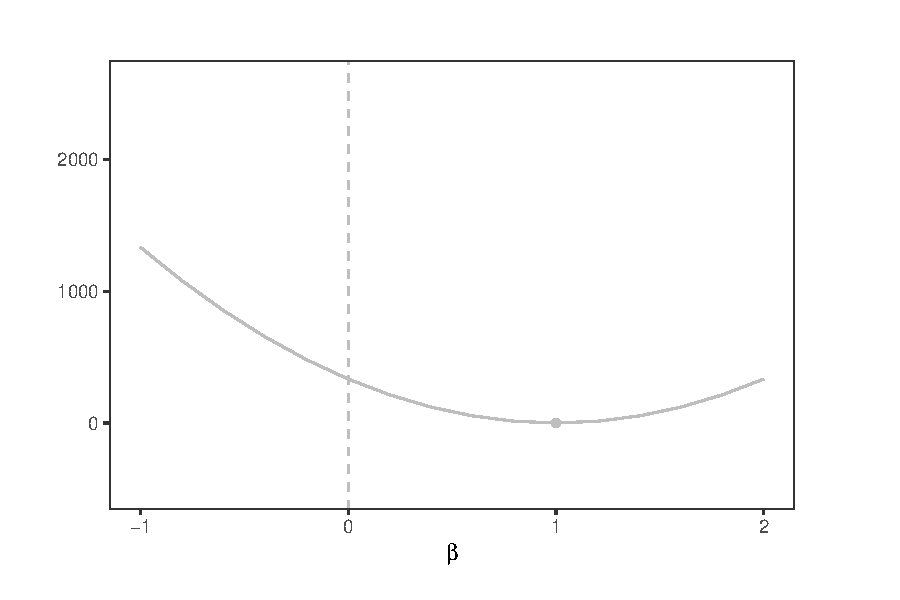
\includegraphics[scale=0.6]{figures/lasso1.pdf}
 \end{figure}




\end{frame}
%----------------------------------------------------------------------%
\begin{frame}[fragile]
\frametitle{Intuición en 1 Dimensión}
\framesubtitle{ $\hat{\beta}>0$}
\footnotesize
\begin{align}
 min_{\beta} E(\beta) = \sum_{i=1}^n (y_i-x_i \beta)^2 + \lambda \beta 
\end{align}
   \begin{figure}[H] \centering
            \captionsetup{justification=centering}
              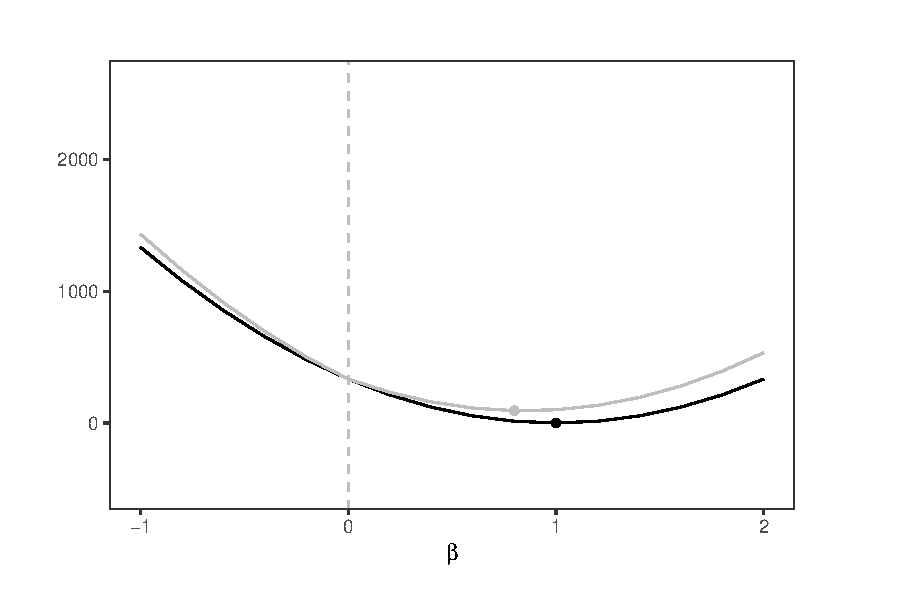
\includegraphics[scale=0.6]{figures/lasso2.pdf}
 \end{figure}




\end{frame}
%----------------------------------------------------------------------%
\begin{frame}[fragile]
\frametitle{Intuición en 1 Dimensión}
\framesubtitle{ $\hat{\beta}>0$}
\footnotesize
\begin{align}
 min_{\beta} E(\beta) = \sum_{i=1}^n (y_i-x_i \beta)^2 + \lambda \beta 
\end{align}

   \begin{figure}[H] \centering
            \captionsetup{justification=centering}
              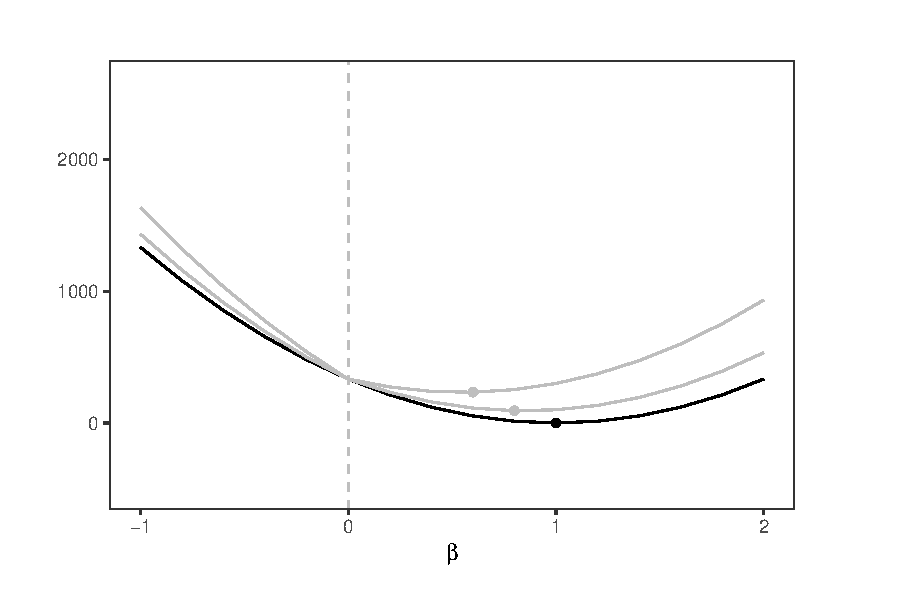
\includegraphics[scale=0.6]{figures/lasso3.pdf}
 \end{figure}




\end{frame}
%----------------------------------------------------------------------%
\begin{frame}[fragile]
\frametitle{Intuición en 1 Dimensión}
\framesubtitle{ $\hat{\beta}>0$}
\footnotesize
\begin{align}
 min_{\beta} E(\beta) = \sum_{i=1}^n (y_i-x_i \beta)^2 + \lambda \beta 
\end{align}

   \begin{figure}[H] \centering
            \captionsetup{justification=centering}
              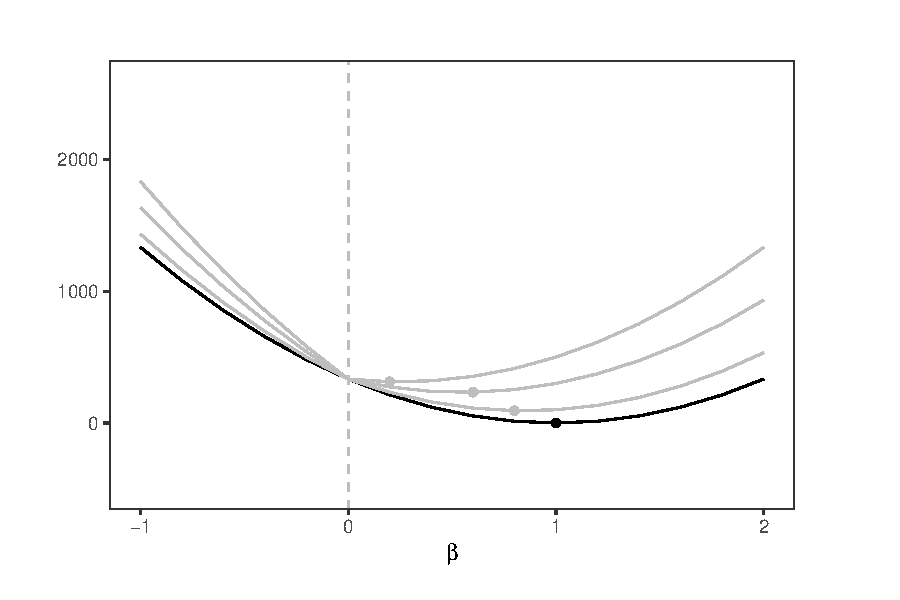
\includegraphics[scale=0.6]{figures/lasso4.pdf}
 \end{figure}





\end{frame}
%----------------------------------------------------------------------%
\begin{frame}[fragile]
\frametitle{Intuición en 1 Dimensión}
\framesubtitle{ $\hat{\beta}>0$}
\footnotesize
\begin{align}
 min_{\beta} E(\beta) = \sum_{i=1}^n (y_i-x_i \beta)^2 + \lambda \beta 
\end{align}

   \begin{figure}[H] \centering
            \captionsetup{justification=centering}
              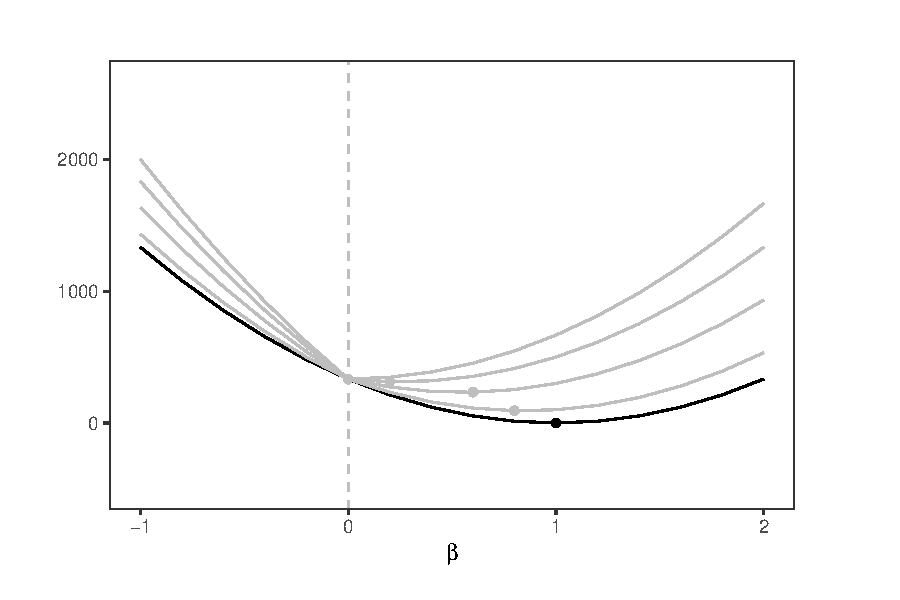
\includegraphics[scale=0.6]{figures/lasso5.pdf}
 \end{figure}


\end{frame}
%----------------------------------------------------------------------%
\begin{frame}[fragile]
\frametitle{Intuición en 1 Dimensión}
\framesubtitle{ $\hat{\beta}>0$}
\footnotesize
\begin{align}
 min_{\beta} E(\beta) = \sum_{i=1}^n (y_i-x_i \beta)^2 + \lambda \beta 
\end{align}

   \begin{figure}[H] \centering
            \captionsetup{justification=centering}
              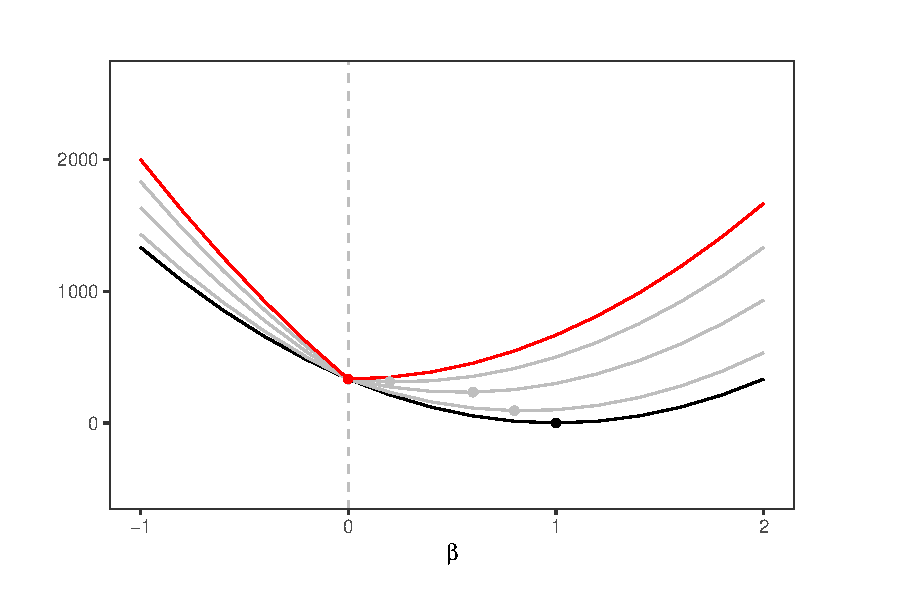
\includegraphics[scale=0.6]{figures/lasso6.pdf}
 \end{figure}


\end{frame}
%----------------------------------------------------------------------%
\begin{frame}[fragile]
\frametitle{Intuición en 1 Dimensión}
\framesubtitle{ $\hat{\beta}>0$}
\footnotesize
\begin{align}
 min_{\beta} E(\beta) = \sum_{i=1}^n (y_i-x_i \beta)^2 + \lambda \beta 
\end{align}

   \begin{figure}[H] \centering
            \captionsetup{justification=centering}
              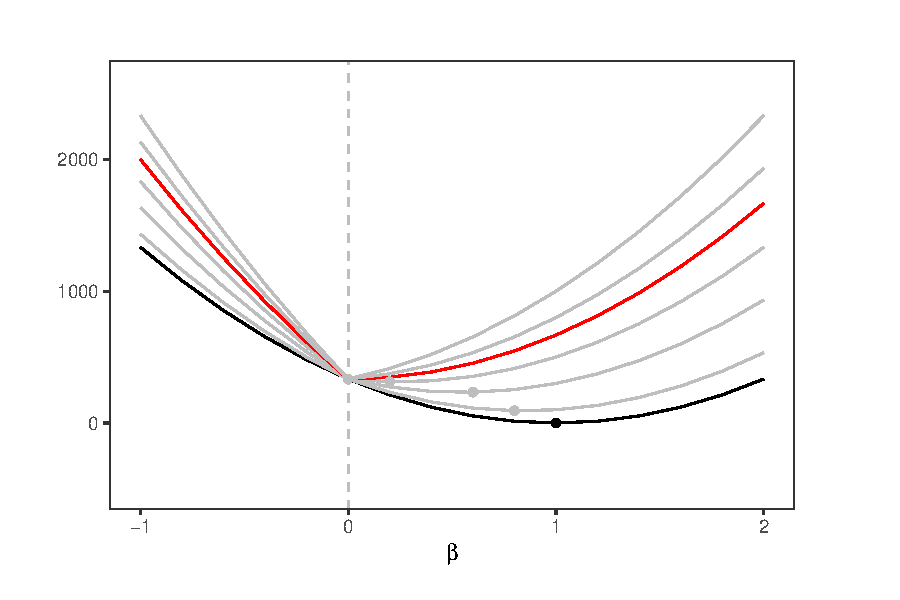
\includegraphics[scale=0.6]{figures/lasso_final.pdf}
 \end{figure}

 \end{frame}
%----------------------------------------------------------------------%
\begin{frame}[fragile]
\frametitle{Ilustración en R}
\begin{figure}[H] \centering
  \centering
  
\includegraphics[scale=0.35]{figures/baticomputer_meme.jpg}
  \\
  \tiny photo from \url{https://www.dailydot.com/parsec/batman-1966-labels-tumblr-twitter-vine/}
\end{figure}

 \end{frame}
%----------------------------------------------------------------------%
\begin{frame}[fragile, t]
\frametitle{Intuición en 1 Dimension}
\framesubtitle{Solución analitica}

\begin{align}
min_{\beta} E(\beta) = \sum_{i=1}^n (y_i-x_i \beta)^2 + \lambda|\beta| 
\end{align}
\pause
\begin{itemize}
\item la solución analítica es 
\end{itemize}

\medskip
\begin{align}
\hat{\beta}_{lasso}=\begin{cases}
0 & \text{\text{si} }\ensuremath{\lambda\geq \lambda^*}\\
\hat{\beta}_{OLS}-\frac{\lambda}{2} & \text{\text{si} }\ensuremath{\lambda<\lambda^*}
\end{cases}
\end{align}


\end{frame}

%----------------------------------------------------------------------%
\begin{frame}[fragile]
\frametitle{Intuición en 2 Dimensiones (Lasso)}
\footnotesize
\begin{align}
     min_{\beta} E(\beta) &= \sum_{i=1}^n (y_i - x_{i1}\beta_1 - x_{i1}\beta_2)^2  \text{ s.a }   \left( |\beta_1| + |\beta_2| \right) \leq c 
  \end{align}

\begin{figure}[H] \centering
            \captionsetup{justification=centering}
              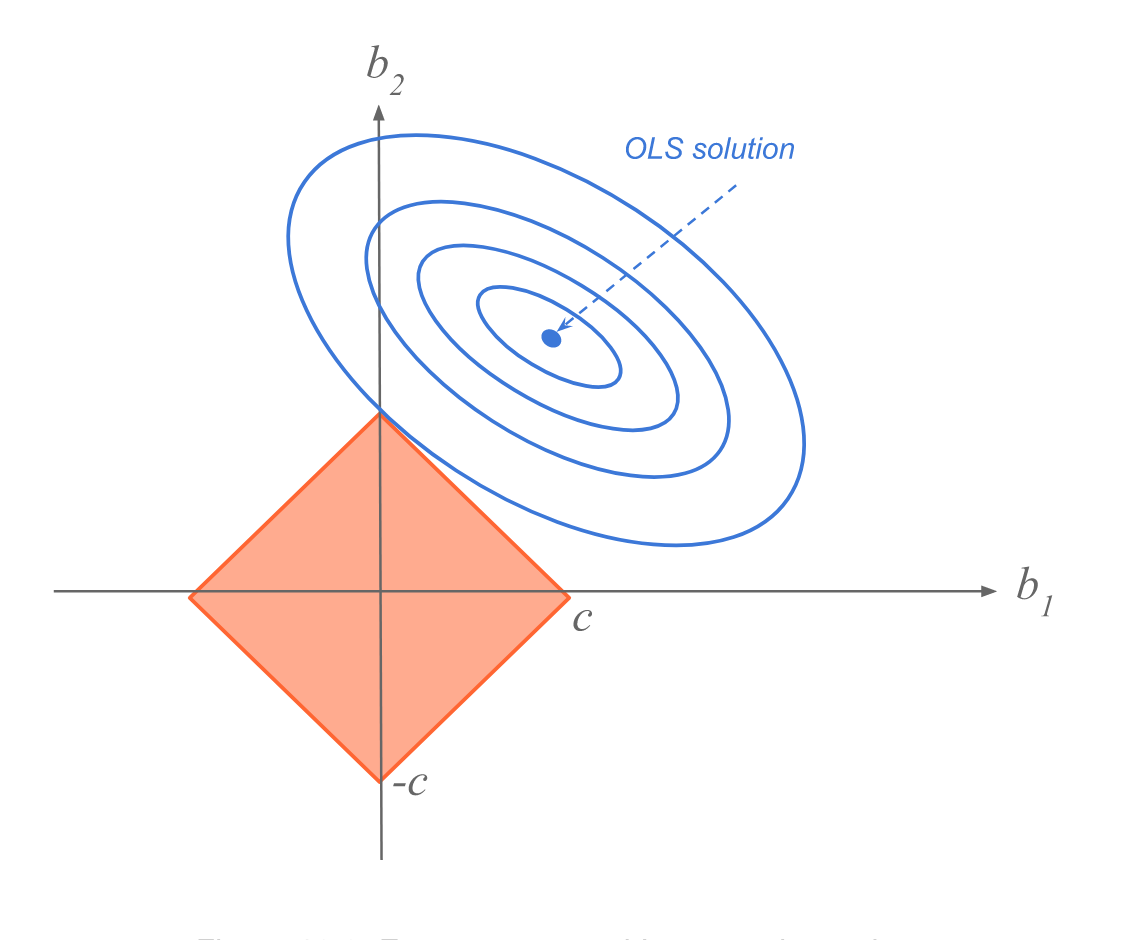
\includegraphics[scale=0.4]{figures/lasso_ridge2}
 
\tiny
Fuente: \url{https://allmodelsarewrong.github.io}
\end{figure}

 \end{frame}


%----------------------------------------------------------------------%
\begin{frame}[fragile]
\frametitle{Example}
\begin{figure}[H] \centering
  \centering
  
\includegraphics[scale=0.35]{figures/baticomputer_meme.jpg}
  \\
  \tiny photo from \url{https://www.dailydot.com/parsec/batman-1966-labels-tumblr-twitter-vine/}
\end{figure}

 \end{frame}

%----------------------------------------------------------------------%
\begin{frame}[fragile]
\frametitle{Resumen}

\begin{itemize}
 \item Ridge y Lasso  son sesgados, pero las disminuciones en varianza pueden compensar estoy y llevar a un MSE menor
 \medskip

 \item Lasso encoje a cero, Ridge no tanto
 \medskip
 \item Importante para aplicación:
\begin{itemize}
  \medskip
 \item Estandarizar los datos 
 \medskip
 \item Como elegimos $\lambda$? \pause $\rightarrow$ Validación cruzada
\end{itemize}
\end{itemize}




 \end{frame}



%----------------------------------------------------------------------%
\section{Familia de regresiones penalizadas}
%----------------------------------------------------------------------%
\begin{frame}[fragile]
\frametitle{Family of penalized regressions}

\footnotesize
\begin{align}
min_{\beta} R(\beta) = \sum_{i=1}^n (y_i-x_i'\beta)^2 + \lambda \sum_{s=2}^p |\beta_s|^p
\end{align}

 \begin{figure}[H] \centering
            \captionsetup{justification=centering}
              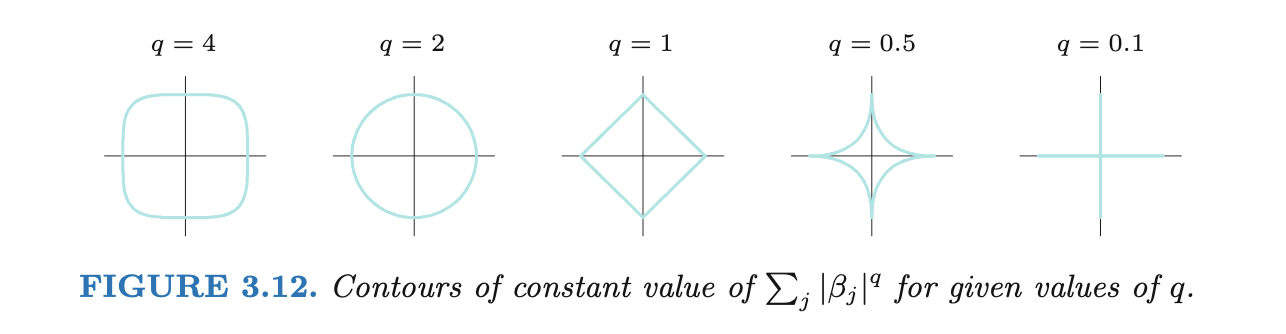
\includegraphics[scale=0.6]{figures/penalties.png}
 \end{figure}


\end{frame}



%----------------------------------------------------------------------%
\section{$k>n$}
%----------------------------------------------------------------------%
\begin{frame}[fragile]
\frametitle{More predictors than observations ($k>n$)}

\begin{itemize}
  \item Objective 1: Accuracy
  \begin{itemize}
    \item Minimize prediction error (in one step) $\rightarrow$ Ridge, Lasso
    \end{itemize}
    \bigskip
  \item Objective 2: Dimensionality
  \begin{itemize}
    \item Reduce the predictor space $\rightarrow$ Lasso's free lunch
    \end{itemize}
\end{itemize}
\bigskip
\bigskip
\begin{itemize}
  \item What happens when we have more predictors than observations ($k>n$)?
  \begin{itemize}
   \item OLS fails
   \medskip
   \item Ridge augments data
   \medskip
   \item and Lasso?
  \end{itemize}
\end{itemize}

\end{frame}


%----------------------------------------------------------------------%
\begin{frame}[fragile]
\frametitle{Lasso when $k>n$}

\begin{itemize}
  \item Lasso works fine in this case
  \medskip
  \item However, there are some issues to keep in mind
  \begin{itemize}
    \medskip
  \item When $k>n$ chooses at most $n$ variables
  \medskip
  \item When we have a group of highly correlated variables, 
  \medskip
    \begin{itemize}
      \item Lasso chooses only one. Makes it unstable for prediction. (Doesn't happen to Ridge)
      \medskip
      \item Ridge shrinks the coefficients of correlated variables toward each other. This makes Ridge ``work'' better than Lasso. ``Work'' in terms of prediction error
    \end{itemize}
  \end{itemize}  
  \medskip
  
\end{itemize}



\end{frame}


%----------------------------------------------------------------------%
\section{Elastic Net}
%----------------------------------------------------------------------%
%----------------------------------------------------------------------%
\begin{frame}[fragile]
\frametitle{Elastic net}



\begin{align}
min_{\beta} EN(\beta) &= \sum_{i=1}^n (y_i-\beta_0 - \sum_{j=1}^p x_{ij}\beta_j)^2  + \lambda\left(\alpha \sum_{j=1}^p |\beta_j| + \frac{(1-\alpha)}{2} \sum_{j=1}^p (\beta_j)^2\right)
\end{align}


\begin{itemize}
 \item Si $\alpha=1$ Lasso
 \medskip
 \item Si $\alpha=0$ Ridge 
\end{itemize}

\end{frame}
%----------------------------------------------------------------------%


\begin{frame}[fragile]
\frametitle{Elastic Net}

\begin{itemize}
\item Elastic net: happy medium. 
  \begin{itemize}
    \item Good job at prediction and selecting variables
  \end{itemize}
\end{itemize}

\begin{align}
min_{\beta} EN(\beta) &= \sum_{i=1}^n (y_i-\beta_0 - \sum_{j=1}^p x_{ij}\beta_j)^2  + \lambda\left(\alpha \sum_{j=1}^p |\beta_j| + \frac{(1-\alpha)}{2} \sum_{j=1}^p (\beta_j)^2\right)
\end{align}


\begin{itemize}
 \item Mixes Ridge and Lasso
 \item Lasso selects predictors
 \item Strict convexity part  of the penalty (ridge) solves the grouping instability problem 
 \item How to choose $(\lambda,\alpha)$? $\rightarrow$ Bidimensional Crossvalidation
 
 \scriptsize
 \item Recomended lecture: Zou, H. \& Hastie, T. (2005)
 \item H.W.: $\beta_{OLS}>0$ one predictor standarized
 \begin{align}
\hat{\beta}_{EN}= \frac{\left(\hat{\beta}_{OLS}-\frac{\lambda_1}{2}\right)_{+}}{1+\lambda_2}
\end{align}
\end{itemize}

%The second term encourages highly correlated features to be averaged, while the first term encourages a sparse solution in the coefficients of these averaged features. The elastic net penalty can be used with any linear model, in particular for regression or classification. pg 662 Elements
\end{frame}



%----------------------------------------------------------------------%
\begin{frame}[fragile]
\frametitle{Example}
\begin{figure}[H] \centering
  \centering
  
\includegraphics[scale=0.35]{figures/baticomputer_meme.jpg}
  \\
  \tiny photo from \url{https://www.dailydot.com/parsec/batman-1966-labels-tumblr-twitter-vine/}
\end{figure}

 \end{frame}


%----------------------------------------------------------------------%
\end{document}
